\documentclass[conference]{IEEEtran}
\IEEEoverridecommandlockouts
% The preceding line is only needed to identify funding in the first footnote. If that is unneeded, please comment it out.
\usepackage{cite}
\usepackage{amsmath,amssymb,amsfonts}
\usepackage{algorithmic}
\usepackage{graphicx}
\usepackage{textcomp}
\usepackage{xcolor}
\usepackage{listings}
\def\BibTeX{{\rm B\kern-.05em{\sc i\kern-.025em b}\kern-.08em
    T\kern-.1667em\lower.7ex\hbox{E}\kern-.125emX}}
\begin{document}

\title{Detect user emotions based on social networks\\
\thanks{Identify applicable funding agency here. If none, delete this.}
}

\author{\IEEEauthorblockN{1\textsuperscript{st} Gerken Jonas}
\IEEEauthorblockA{\textit{Hochschule Hamm-Lippstadt} \\
jonas.gerken@stud.hshl.de}
}

\maketitle

\begin{abstract}
\newline
Die folgende Ausarbeitung befasst sich mit der Erkennung von Emotionen basierend auf Sozialen Netzwerken.
Zunächst wird in der Motivation erläutert was eine Emotion umfasst, wo Emotionen heute in Sozialen Netzen zu finden sind und wo Emotionsanalyse angewendet werden kann.
Weiter werden die beiden Emotionsmodelle Ekman und das OCC-Modell beschrieben.
Im nächsten Kapitel werden die drei verschiedene Ansätze Keyword based, Learning based und Hybrid based erläutert, welche für die Emotionserkennung im Text benutzt werden können.
Des weiteren wird spezifischer auf die Emotionsanalyse in Sozialen Netzwerken eingegangen. Hier wird zu nächst die Emotionsanalyse erläutert und was es dort zu beachten gibt. Zudem werden zwei weitere Methoden zur Emotionsanalyse beschrieben.
Als nächstes wird beschrieben, wie Twitter Emotionen während eines Erbebens analysiert werden. Hierzu werden die drei Ansätze: Textual keyword spotting, Rule-based linguistic und der Feature-based classification Ansatz erläutert.
Dazu wird noch auf ähnliche Arbeiten eingegangen, die sich auf andere Krisenkontexte wie Hurrikans und Gasexplosionen bezogen.
Danach wird auf die Analyse von suizidalen Texten eingegangen. Hier wird zunächst die Geschichte der Analyse von suizidalen Texten erläutert. Des weiteren geht es um die maschinellen Lerntechniken zur Analyse solcher Texte.
Im nächsten Abschnitt wird ein Beispiel Projekt zur Emotionsanalyse dargestellt.
\end{abstract}

\section{Motivation}
Emotionen umfassen Gefühle, Erfahrungen, Physiologie, Verhalten, Kognitionen und Konzeptualisierungen. Laut WordNet Search 3.0 ist eine Emotion "jedes starke Gefühl". Wikipedia definiert eine Emotion als "einen mentalen und physiologischen Zustand, der mit einer Vielzahl von Gefühlen, Gedanken und Verhaltensweisen verbunden ist". Wir stellen fest, dass der Aspekt des Fühlens häufig ist und durch begleitende physiologische Veränderungen und Mimik charakterisiert werden kann.\cite{b2}
Mit der schnellen Entwicklung der Plattformen für soziale Online-Netzwerke (OSNs) (z. B. Twitter, Facebook usw.) ist das Ausdrücken von Emotionen oder das Teilen bedeutungsvoller Momente mit Freunden in OSNs zu täglichen Aktivitäten der Menschen geworden.
Viele veröffentlichte Inhalte in OSNs bieten eine gute Gelegenheit, die Emotionen der Benutzer zu untersuchen, und ermöglichen so die schnelle Entwicklung emotionsbewusster Anwendungen.
Beispielsweise kann ein Aktivitätsmanagementsystem oder ein personalisiertes Werbesystem wertvolle Vorschläge machen oder auf emotionale Weise einen Zeitplan erstellen. Ein personalisiertes Empfehlungssystem kann personalisierte Produkte, Filme oder Songs entsprechend den aktuellen Emotionen des Einzelnen empfehlen. 
Bei öffentlichen Notfällen wie Erdbeben oder Pandemien kann die Erkennung von Emotionen in Online Social Networks s zur Überwachung der öffentlichen Meinung verwendet werden, die die Entscheidungsfindung der Regierung unterstützt.\cite{b1}

\section{Emotionsmodelle}
Hier werden kurz die Emotionsmodelle von Ekman und das OCC-Modell (Ortony/Clore/Collins) beschrieben. 
Emotionsmodelle schreiben das notwendige Wissen vor, um Ereignisse einzuschätzen. Ekmans Emotionsmodell besteht aus Traurigkeit, Glück, Wut, Angst, Ekel und Überraschung. Es wurde in Systemen verwendet, die Gesichtsausdrücke im Zusammenhang mit diesen emotionalen Zuständen erkennen. In dieser Ausarbeitung wird auch textbasierend verwendet. Das OCC-Modell stellt Emotionen dar, die im Allgemeinen von einem Agenten ausgedrückt werden. Es umfasst 22 Emotionskategorien, die den Menschen im Allgemeinen modellieren sollen. Es basiert auf der Prämisse, dass Emotionen keine sprachlichen Dinge sind, aber der am leichtesten zugängliche nicht-phänomenale Zugang zu Menschen ist durch Sprache.

Der Hauptvorteil der Verwendung des OCC-Modells besteht darin, dass es eine Spezifikation für verschiedene Arten von Emotionen mit einer relativ kulturfreien Grundlage bietet. Dadurch entfällt die Notwendigkeit, Emotionen basierend auf bestimmten Wörtern zu studieren, sondern als Klassen von zugrunde liegenden Emotionstypen. Mit anderen Worten, es ist eine Theorie der Emotionen
und keine Theorie der Sprache der Emotionen. Die sechs Emotionstypen in Ekmans Modell erscheinen im OCC-Modell, weil die im ersten Modell spezifizierten spezifischen Schlüsselwörter auf spezifische Emotionstypen abgebildet werden können, die unter Verwendung von Token (zB Glück, Traurigkeit, Wut, Ekel, Überraschung und Angst) im letzteren spezifiziert werden. Die OCC
Emotionstypen sind: Glücklich, Entschuldigung, Groll, Schadenfreude, Hoffnung, Angst, Bestaetigte Angst, Erleichterung, Enttaeuschung, Stolz, Selbstvorwurf, Wertschaetzung, Vorwurf, Dankbarkeit, Wut, Befriedigung, Reue, Zuneigung, Abneigung, Schande.\cite{b2}

\section{Ansätze für Emotionserkennung im Text}
Drei Ansätze dominieren derzeit die Aufgabe der Emotionserkennung; Keyword-basierter, lernbasierter und hybridbasierter Ansatz. Diese bestehen hauptsächlich aus syntaktischen (z. B. N-Grammen, Pos-Tags, Phrasenmustern) und semantischen (z. B. Synonymsätzen) ausgewählten Merkmalen, um Emotionen zu erkennen. Es kann beispielweise WordNet 1.6 verwendet werden, um
Synonymsätze (d. h. Synsets gemäß der wordNet-Terminologie) aus Emotions-Seed-Wörtern zu extrahieren, die nach ihrem Wortarten-Tag (pos) gruppiert sind. Das wird verwendet, um ein affektives Lexikon zu erstellen, indem die Open Mind Common Sense Knowledge Base (OMCS) als wissensreiche linguistische Ressource verwendet wird, da wordNet allein eine allgemeine
Bedeutung von Wörtern bereitstellt. In diesem Abschnitt wird jeder Ansatz mit Schwerpunkt auf deren Vor- und Nachteile kurz Beschrieben.\cite{b2}

\subsection{Keyword based approach}
Dieser Ansatz beruht vollständig auf dem Vorhandensein von Schlüsselwörtern und kann eine Vorverarbeitung mit einem Parser und einem Emotionswörterbuch beinhalten. Es ist einfach zu implementieren, intuitiv und unkompliziert, da es das Identifizieren von Wörtern beinhaltet, nach denen im Text gesucht werden soll. Dies wurde in Echtzeit-Chat-Systemen angewendet. Es ist jedoch domänenspezifisch, beruht auf dem Vorhandensein von Schlüsselwörtern für genaue Ergebnisse und erfordert eine Vorverarbeitung für verbesserte Genauigkeit.\cite{b2}


\subsection{Learning based approach}
Dieser Ansatz verwendet einen trainierten Klassifikator, um Eingabetext in Emotionsklassen zu kategorisieren, indem Schlüsselwörter als Merkmale verwendet werden. Es ist einfacher und schneller, sich an Domänenänderungen anzupassen, da es schnell neue Funktionen aus Korpora(Datasets) lernen kann, indem es einen großen Trainingssatz an einen maschinellen Lernalgorithmus zum Erstellen
eines Klassifizierungsmodells liefert. Der Erwerb großer Korpora ist jedoch möglicherweise nicht immer machbar. Trotzdem erleichtert dies die einfache Implementierung von Klassifikatoren durch novizen, die dann das gelernte Modell auf neue Instanzen anwenden können. Der größte Nachteil dieses Ansatzes besteht darin, dass er zu unscharfen Grenzen zwischen Emotionsklassen und
einer fehlenden Kontextanalyse führt. Zur Klärung der Klassifikationsaufgabe wird hier die Support Vector Machine (SVM) vorgestellt. SVM ist ein allgemein verwendeter Algorithmus, der auf der statistischen Lerntheorie basiert. Es hat sich in vielen Bereichen (Bioinformatik, Text-,
Bilderkennung) empirisch gut bewährt. SVM nimmt eine gleichmäßige Verteilung zwischen positiven und negativen Trainingsbeispielen aus der SVM-Hyperebene an, wie in 1 gezeigt. Die Klassifizierung basiert auf dem Randabstand von der Entscheidungshyperebene (h) zu den positiven und negativen Trainingsbeispielen.\cite{b2}

\begin{figure}[h]
	\centering
	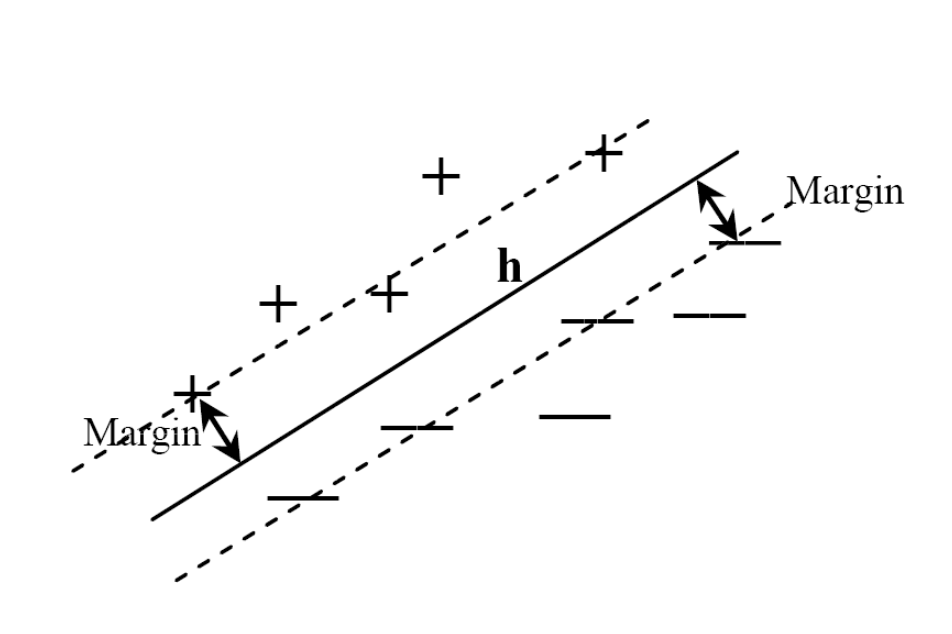
\includegraphics[width=8cm]{svm}
	\caption{Verteilung gerader Ränder von svm-Hyperebene (h)}
\end{figure}

\newpage
\subsection{Hybrid based approach}
Dieser Ansatz besteht aus einer Kombination der schlüsselwortbasierten Implementierung und der lernbasierten Implementierung. Der Hauptvorteil dieses Ansatzes besteht darin, dass er durch das Training einer Kombination von Klassifikatoren und das Hinzufügen wissensreicher linguistischer Informationen aus Wörterbüchern und Thesauri eine höhere Genauigkeit erzielen kann. Dies hat
den Vorteil, dass es die hohen Kosten ausgleicht, die mit der Verwendung menschlicher Indexer für Informationsabrufaufgaben verbunden sind, und die bei der Integration verschiedener lexikalischer Ressourcen auftretende Komplexität minimiert.\cite{b2}

\section{Emotionsanalyse in OnlineSocialNetwork-Texten}
Emotionsanalyse oder Sentimentanalyse haben in letzter Zeit immer mehr Forscher interessiert.
Das Ziel der Sentimentanalyse war in der Regel die Vorhersage der Polarität (positiv, negativ oder neutral) eines Objekts, die bei der Analyse von Filmrezensionen, Produktansichten, Meinungsforschung usw. untersucht wurde. Emotionserkennung wird normalerweise als feinkörnige Sentimentanalyse angesehen. Die Emotionsanalyse kann mehr Kategorien umfassen als die
Sentimentanalyse zur Polaritätsvorhersage. Über die Emotionserkennung im traditionellen menschlichen sozialen Netzwerk hat Fowler behauptet, dass sich Glück oder Depression von Individuum zu Individuum ausbreiten können, basierend auf klinischen Studien. Die Datenmenge, die von traditionellen menschlichen sozialen Netzwerken gesammelt werden, könnte jedoch sehr begrenzt sein. Dank der schnellen Entwicklung von sozialen Online-Medien wie Facebook, Twitter können viel mehr Daten für die Analyse von Forschern gewonnen werden. Moodcast beispielsweise leitete die Emotionen von Einzelpersonen ab, indem der soziale Einfluss, die zeitliche Korrelation und die Standortinformationen als Merkmale berücksichtigt wurden. Yanget hat die
Kommentar Informationen und visuellen Merkmale von Bildern gemeinsam modelliert, um die Leistung bei der Erkennung von Emotionen von Personen anhand von Bildern weiter zu verbessern. Wanget schlug ein Emotionsvorhersagemodell vor, indem der emotionale Einfluss von Einzelpersonen in sozialen Online-Bildnetzwerken wie Flicker quantifiziert wurde. Zhanet al. schlug einen geräuschbewussten Klassifizierungsrahmen für das Crowdsourcing von Emotionserkennungsdatensätzen in OSNs vor. Tanget al. entwarf ein Emotionsübergangsmodell für versteckte Themen, um sowohl die Emotion auf Dokumentebene als auch die Emotion auf Satzebene zu erkennen.

Offensichtlich ist die Erkennung von Emotionen in OSNs wie Facebook oder Twitter immer ein heißes Thema. Im Allgemeinen wurden zwei Hauptmethoden für die Emotionserkennung in OSNs weit verbreitet: 1) lexikonbasierte Methode und 2) maschinelle Lernmethode. Das Ziel der lexikonbasierten Methode ist es, Emotionen aus Texten zu extrahieren, die auf einigen bekannten
Wörterbüchern wie den LIWC-Wörterbüchern basieren. Es wurden sechs Arten von Stimmungszuständen (Depression, Anspannung, Vitalität, Wut, Verwirrung, Müdigkeit) aus Twitter-Texten unter Verwendung des LIWC-Wörterbuchs extrahiert und die Ergebnisse wurden mit mehreren wichtigen Ereignissen vergleichen. Die lexikonbasierten Methoden sind jedoch stark abhängig von der Quantität und Qualität der Wörter in den Wörterbüchern.
\\ 
Die auf maschinellem Lernen basierenden Methoden erkennen Emotionen normalerweise, indem sie Arten von Merkmalen aus Inhalten in OSNs extrahieren und dann Gefühle oder Emotionen unter Verwendung verschiedener Arten von Klassifizierungs- oder Regressionsmodellen vorhersagen. Im Detail analysierten Vo und Collier die Emotionen von Personen in Erdbebensituationen auf Twitter und schlugen dann Arten von Emotionskategorien für die Erdbebensituationen vor, darunter Unannehmlichkeiten, Ruhe, Angst, Traurigkeit, Erleichterung und Angst. Zudem wurden Emotionen auf Satzebene in Twitter analysiert und ein Klassifikator gebaut, um die Emotionsklasse der veröffentlichten Tweets zu bestimmen. Eine weietre Idee war das trainieren von überwachten Klassifikatoren, um die durch Twitter-Nachrichten ausgedrückten Emotionen automatisch zu erkennen und zu klassifizieren, wobei hochdimensionale und spärliche Merkmalsvektoren vermieden werden. Neben dem Training von Emotionsklassifikatoren wurde der Sprachstil des verwendeten Korpus zum Ausdruck von Emotionen analysiert. Deyuet al. erlernte Emotionsverteilungen aus Social-Media-Texten, indem die Beziehungen von Emotionen basierend auf dem Plutchik-Emotionsrad erfasst wurden. Die meiste vorhandene Literatur betrachtet jedoch nur die Erkennung einzelner Emotionen, wobei jedoch ignoriert wird, dass mehrere
Emotionen koexistieren könnten. Anders als in der bestehenden Literatur wird  die Erkennung der multiplen Emotionen in OSNs betrachtet, was in der Vergangenheit nicht oft der Fall war.\cite{b1}
\begin{figure}[h]
	\centering
	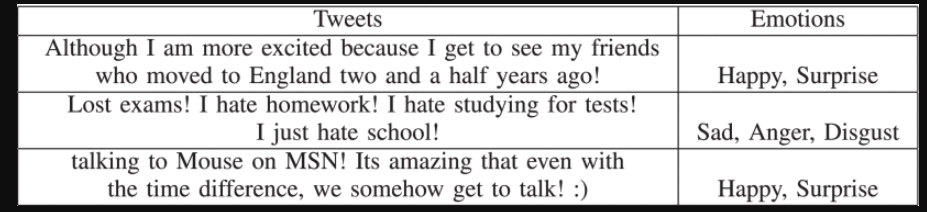
\includegraphics[width=9cm]{Tweets}
	\caption{Tweet mit mehreren Emotionen}
\end{figure}



\section{Twitter Emotionen bei Erdbeben}
Um Emotionen während eines Erdbebens zu analysieren, besteht die erste wichtige Aufgabe darin, Tweets zu identifizieren, die sich auf Erdbeben beziehen. Diese Erdbeben betroffenen Tweets können in den Twitter-Daten durch ein vorgeschlagenes überwachtes Klassifizierungsverfahren erkannt werden. Für die Emotionsanalyseaufgabe wurden Trainingsdaten zu den Emotionen "Ruhe, Unlust, Traurigkeit, Sorge, Angst und Erleichterung" kommentiert. Ein weiteres Verfahren verwenden eine andere überwachte Methode zur Emotionserkennung und manuell wird dann die kategorisierten Emotionen in das Zeitintervall jedes Erdbebens eingetragen. Für beide Klassifizierungsverfahren werden verschiedene Features und Machine-Learning-Modelle verwendet, um die besten Features und Modelle
auszuwählen. Dem Dokument zufolge war das die erste Forschung zur Emotionserkennung und -verfolgung für Twitter-Daten in Erdbebensituationen, während die Erdbebenbezogenen Twitter-Analysearbeiten die emotionalen Aspekte der Benutzer nicht berücksichtigten. Dennoch sind die Emotionsauswahl und die Klassifikationsmethoden mit entsprechenden Features für
japanische Social Media die ersten Beiträge für Twitter-Emotionsanalyseanwendungen.


Sentimentanalyse und Emotionsanalyse sind die Aufgaben, die Einstellungs- und Emotionsklassen des untersuchten Dokuments zu identifizieren . Das hier verwendete Wort Dokument hat eine allgemeine Bedeutung, da es sich auf eine sprachliche Einheit beziehen kann, die einen einzelnen Satz, einen Absatz und ein Dokument mit vielen Ansätzen umfasst. Es gibt drei Hauptansätze, die für
die Identifikation von Emotionen und Einstellungen verwendet werden:

\subsection{Textual keyword spotting approach}
Verwendung einer Reihe von Emotionswörtern
meist Adjektive und Adverbien, die durch spezifische lexikalische Ressourcen definiert werden
wie Google Profiles of Mood States , Linguistic Inquiry und Word
Zählen Sie Wörterbücher , um Dokumente wie Tweets und den Facebook-Status auszuwählen, die solche Schlüsselwörter in unterschiedlichen Emotionen enthalten. Diese
Methode wird aufgrund des großen Umfangs und der
Rauschen von Daten aus sozialen Netzwerken, da es eine beträchtliche Menge an
irrelevante Dokumenten gibt. Während dieser Ansatz direkt auf Englische Tweets ohne Modifikation von Adjektiven und Adverbien anwendbar ist, ist es schwierig für Japanisch, eine agglutinierende Sprache anzuwenden.

\subsection{Rule-based linguistic approach}
Jeder Satz wird in Etappen verarbeitet,
einschließlich symbolischer Hinweise, Abkürzungen, Satzanalyse und Analyse auf Wort-/Phrasen-/Satzebene. Dieser regelbasierte Ansatz ist oft aufgrund der Vielfalt der natürlichen Sprache, insbesondere der Sprache in sozialen Netzwerken Eingeschränkt.

\subsection{Feature-based classification approach}
Dieser empirische Ansatz
wurde von den ersten Anwendungen der Stimmungsanalyse im Film 
Rezensionen zu aktuellen Sentiment- und Emotionsanalyseanwendungen auf
sozialen Medien verwendet.  Es wird die Bestimmung der Emotion von einer
Spracheinheit betrachtet, die ein Mehrklassenklassifikationsproblem ist. Dies beaufsichtigt
Lernansatz generiert eine Funktion, die linguistische Einheiten auf
die gewünschte Emotion durch Betrachtung der aus der Sprache abgeleiteten Merkmale
unit-emotion Beispiele für die Funktion. Die Merkmale können n-Gramm sein,
Wortschatz oder Twitter-Funktionen wie Re-Tweets, Hashtags, Antworten,
Satzzeichen und Emoticons.
\newline

\subsection{Ähnliche Arbeiten}
Es gibt einige ähnliche Arbeiten zur Sentimentanalyse in Krisenkontexten
zu Erdbebenereignissen, wie Hurrikane oder Gasexplosionen.
Diese Werke verwenden auch die merkmalsbasierte Klassifizierungsmethode für Englische
Sentimentanalysen. Es wurde mit Funktionen experimentiert: zwei Tokenizer-Alternativen, Entfernung von Stoppwörtern, Frequenzbeschneidung, Sorgenlexikon,
Humorlexikon und Emoticon; und Klassifikatoren: Maximale Entropie, Entscheidungsbaum und Naive Bayes, um die besten Funktionen und das beste Modell auszuwählen.
Klassifizierung von Tweets zu Hurrikan betroffen oder unbeteiligten. Nagy
und Stamberger kombinieren die verfügbaren englischen Sentiment-Daten bestehend aus SentiWordNet, Emoticons, AFNN zur Klassifizierung nach Bayesian
Netzwerk.

Viele englischsprachige Untersuchungen zur Emotionsanalyse klassifizieren Dokumente
zu Ekmans 6 Grundemotionen: Überraschung, Glück, Wut, Angst, Ekel und Traurigkeit. Inzwischen basieren einige japanische Werke auf Nakamuras japanischem Emotionswörterbuch mit 10 Emotionstypen: Aufregung, Scham, Freude, Vorliebe, Abneigung, Trauer, Wut, Überraschung, Angst und
Linderung; und Tokuhisa et al. Verwenden Sie 10 Emotionsklassen: Glück, Angenehmheit, Enttäuschung, Unlust, Einsamkeit, Traurigkeit, Wut,
Angst, Angst und Erleichterung aus dem Teramura-Wörterbuch. Es ist klar, dass
die von Tokuhisa et al. sind getrennter als die von Ekman
Emotionen. Außerdem sind Nakamuras Emotionen Aufregung, Freude, Zuneigung ziemlich ähnlich und zusammen mit Scham sind sie nicht angemessen in
Erdbeben Kontexte.\cite{b3}

\section{Analyse suizidaler Texte}
Die linguistische Analyse suizidaler Texte hat eine lange Geschichte, die bereits 1957 begann. Der Großteil dieser Forschung basierte auf einem Korpus von 66 von Shneidman gesammelten Abschiedsbriefen, halb echt und halb simuliert, und die Aufgabe bestand darin, Merkmale zu identifizieren, um zwischen echten und gefälschten Notizen zu unterscheiden. Frühe Arbeiten konzentrierten sich hauptsächlich auf die manuelle Analyse und Erkennung solcher Merkmale, z.B. indem man sich auf Techniken der Diskursanalyse stützt oder sich auf oberflächliche Textmerkmale wie die Verwendung von Modalen und Hilfsstoffen, die Wahl von Verben und Adverbien usw.. In jüngster Zeit wurde eine Tendez beobachtet, die sich auch auf automatische Korpusanalysetechniken zur Erkennung von Suizidbotschaften zu konzentrieren. Es wurden zwei Korpora von Abschiedsbriefen untersucht, um den typischen Abschiedsbrief zu definieren, indem Wortgebrauch und semantische Konzepte quantifiziert wurden. Als erstes experimentierten Pestian, Nasrallah, Matykiewicz, Bennett u. Leenaars mit maschinellen Lerntechniken zur automatischen Klassifikation von Abschiedsbriefen. Diese Techniken zeigten, dass automatische Systeme Psychologen bei der Trennung echter von gefälschten Notizen übertreffen könnten. Da ist aber wichtig zu bestimmen, was genau eine Notiz zu einem echten Abschiedsbrief macht unabhängig von den Merkmalen der erfragten Notizen oder den Unterscheidungsmerkmalen zwischen beiden Arten von Notizen.
Im Rahmen der i2b2 NLP 5 Challenge 2011 zur Emotionsklassifizierung in Abschiedsbriefen, die auf suizidales Verhalten hinweisen und wie sie automatisch gefunden werden können. Bei der automatischen Emotionserkennung und -klassifizierung kann auf die jüngsten Fortschritte im NLP und maschinellen Lernen zurückgegriffen werden. Obwohl sich die NLP-Forschungsgemeinschaft seit langem auf die sachlichen Aspekte der Inhaltsanalyse konzentriert, hat sich die Menge an Informationen, die derzeit in sozialen Medien produziert werden, auch das Interesse an der automatischen Analyse von Emotionen und Meinungen vergrößert. 
Ein NLP-System, das sowohl sachliche Informationen als auch Meinungen, Gefühle und Überzeugungen aus Texten extrahiert, schafft viele Möglichkeiten für Organisationen und Einzelpersonen: beim Benchmarking von Produkten, bei der Beratung von Einzelpersonen bei ihren Einkäufen, zur Vorhersage oder Messung an den Aktienmärkten oder in der Politik, aber auch zur Detektion von Emotionen in Abschiedsbriefen.\cite{b4}

Bisher konzentrierten sich die meisten Arbeiten darauf, herauszufinden, ob ein bestimmtes Objekt (Person, Produkt, Organisation, Ereignis usw.), die von einer bestimmten Quelle(dh einer Person, einer Organisation, einer Gemeinschaft, Menschen in allgemein usw.) positiv oder negativ bewertet wurden. Dieser Aufgabe wurden viele Namen gegeben, von Opinion Mining, Sentiment Analysis, Review Mining, Einstellungsanalyse, Appraisal Extraction und vielen anderen. Zur Lösung der Aufgabe wurden verschiedene Techniken vorgeschlagen, von einfachen lexikonbasierten Systemen, die die Polarität einer bestimmten Texteinheit durch Zählen der Anzahl positiver und negativer Wörter bestimmen, bis hin zu überwachten maschinellen Lerntechniken, die auf annotierten Korpora beruhen. Beispiele für überwachte maschinelle Lernansätze sind naive Bayes, Support Vector Machines, Memory-based Learning und Hidden Markov Models. Um Meinungen oder Emotionen auf Dokumenten-, Satz- und Satzebene automatisch zu extrahieren und zu klassifizieren, können verschiedene Arten von Informationsquellen (Features) verwendet werden.\cite{b4}

Es wird allgemein angenommen, dass die semantischen Eigenschaften einzelner Wörter gute Prädiktoren für die semantischen Eigenschaften der Phrase oder des Textes sind, die sie enthalten, weshalb viel Aufwand in die manuelle, halbautomatische und automatische Entwicklung von Listen investiert, wurde von Worten, die auf Stimmung hinweisen. Lexikonbasierte Sentiment-Mining-Systeme nutzen die in den Daten enthaltenen lexikalischen Informationen (z. B. Unigramme, Bigramme usw.) und externe Sentiment-Lexika, um für einen bestimmten Text, Satz oder Ausdruck zu bestimmen, ob er positiv, negativ oder neutral ist. Man könnte erwarten, dass ein Abschiedsbrief Wörter enthält, die sich auf Selbstmord bezieht. Zum Beispiel wurden Wörterbücher mit Suizid-bezogenen Schlüsselwörtern erfolgreich für die Erkennung von Suizid-Blogs verwendet, obwohl viele falsch positive Ergebnisse gemeldet wurden (z. B. hat jemand in Ihrer Nähe Selbstmord begangen? als Inhalt einer selbstmörderischen Person angesehen werden). Der Ausdruck von Gefühlen kann nicht nur in einzelnen Wörtern liegen, sondern auch in Kombinationen von Wörtern (z. B. ich würde mich nie umbringen versus ich werde mich umbringen oder das Verb hängen, um sich aufzuhängen versus Weihnachtslichter aufzuhängen). Um Verneinungen, verschiedene Wortbedeutungen usw. zu erfassen, können spezifische NLP-Komponenten andere relevante Funktionen bereitstellen, wie z. B. Named-Entity-Erkenner für die Objektidentifikation, Synonymie-Erkennungssysteme, Parser, Wortsinn-Disambiguierungssysteme, Koreferenzresolver zur Themenidentifikation, Systeme zur Negations-Scope-Erkennung usw.\cite{b4}

Die Analyse selbst kann auf verschiedenen Ebenen durchgeführt werden. Grobkörniges Opinion Mining auf Dokumentebene zielt darauf ab, die allgemeinen Stimmungseigenschaften eines Textes zu bestimmen, indem es als positiv, negativ oder neutral klassifiziert wird, und wurde umfassend untersucht. Die feingranulare Sentimentanalyse beschäftigt sich mit Sätzen und Klauseln. Es kann die Ziele von Meinungen auf Entitäts- und Aspektebene identifizieren, den Fokus auf die automatische Klassifizierung der Meinungsintensität legen oder auf die feinkörnige Unterscheidung zwischen verschiedenen Arten von Emotionen. Diese Forschungsrichtung wurde beispielsweise von (Strapparava u. Mihalcea, 2007) oder (Bellegarda, 2010) untersucht, die zwischen den 6 universellen Emotionen unterschieden, wie sie von (Ekman, 1993) vorgeschlagen wurden: Wut, Ekel, Angst, Traurigkeit, Freude und Überraschung. Sowohl die niedrigen Übereinstimmungswerte zwischen den Annotatoren als auch die große Lücke zwischen den manuellen Annotationen und den berichteten Systemergebnissen zeigen, dass im Bereich der Emotionserkennung viel Raum für Verbesserungen besteht.\cite{b4}

\section{Projekt}
Am Anfang des Projekts habe ich eine Requirement Tabelle erstellt.
\begin{figure}[h]
	\centering
	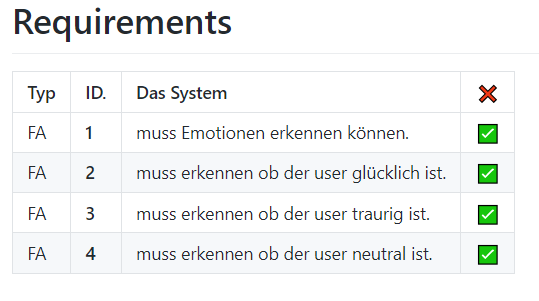
\includegraphics[width=10cm]{Requirements}
	\caption{Requirements}
\end{figure}

Danach habe ich die aus den Requirements ein Use Case erstellt.
\begin{figure}[h]
	\centering
	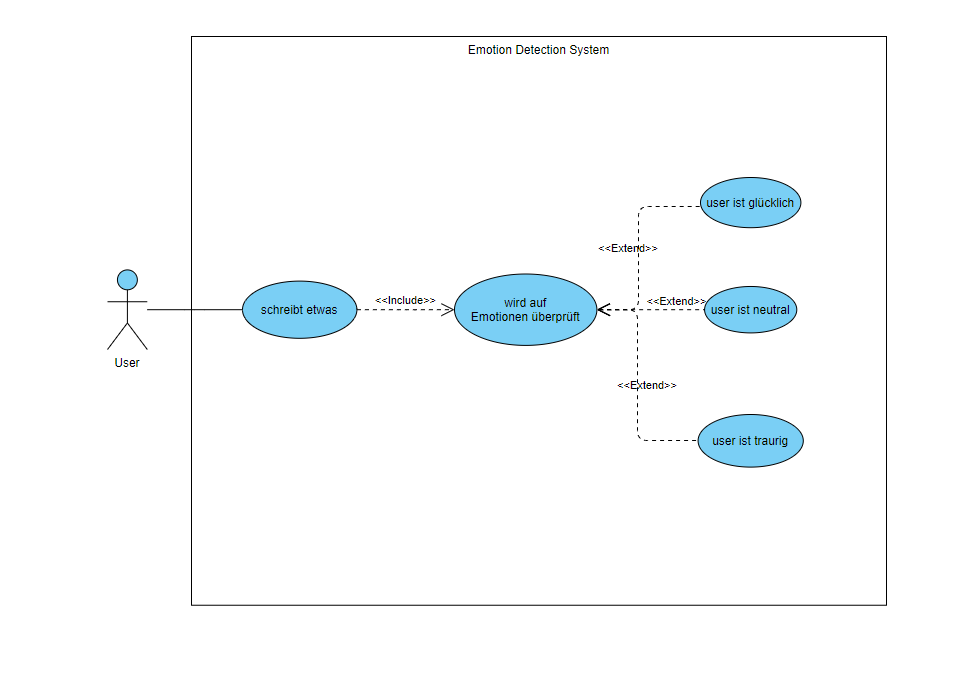
\includegraphics[width=10cm]{UseCase}
	\caption{Use Case}
\end{figure}

Für das Projekt "Detect user emotions based on social networks" wird das Programm sklearn und jupyter lab verwendet. 
Sklearn ist eine Software-Bibliothek zum maschinellen Lernen für die Programmiersprache Python. Mit diesem Befehl 
pip install numpy pandas sklearn wird über die Windows Console sklearn installiert.
Die pandas Programmbiblithek für Python wird verwendet, um die Daten zu Verwalten und zu analysieren.

JupyterLab ist eine webbasierte interaktive Entwicklungsumgebung für Jupyter-Notebooks, -Code und -Daten. JupyterLab muss zunächst über die Website heruntergeladen und installiert werden und kann dann über den Speicherort ausgeführt werden C:,Users,DataFlair,jupyter lab.

Dieses Python-Projekt zur Erkennung von Emotionen befasst sich mit verschiedenen Emotionen, die in Social Media Netzwerken auftreten können. Mit sklearn wird ein TfidfVectorizer auf unserem Datensatz erstellt. Dann wird ein PassiveAggressive Classifier initialisiert und dann wird das Modell angepasst. Am Ende sagt ein Genauigkeitswert und eine Confusion Matrix an, wie gut das Modell ist.

Was ist ein TfidfVectorizer?
TF (Begriffshäufigkeit): Die Häufigkeit, mit der ein Wort in einem Dokument vorkommt, ist seine Begriffshäufigkeit. Ein höherer Wert bedeutet, dass ein Begriff häufiger vorkommt als andere. Daher ist das Dokument eine gute Übereinstimmung, wenn der Begriff Teil der Suchbegriffe ist.
IDF (Inverse Document Frequency): Wörter, die in einem Dokument häufig vorkommen, aber auch in vielen anderen häufig vorkommen, können irrelevant sein. IDF ist ein Maß dafür, wie wichtig ein Begriff im gesamten Dataset (Korpus) ist.
Der TfidfVectorizer konvertiert eine Sammlung von Rohdokumenten in eine Matrix von TF-IDF-Funktionen.

Was ist ein PassiveAggressiveClassifier?
Passive Aggressive Algorithmen sind Online-Lernalgorithmen. Ein solcher Algorithmus bleibt für ein korrektes Klassifizierungsergebnis passiv und wird im Falle einer Fehlberechnung, Aktualisierung und Anpassung aggressiv. Im Gegensatz zu den meisten anderen Algorithmen konvergiert er nicht. Sein Zweck besteht darin, Aktualisierungen vorzunehmen, die den Verlust korrigieren und eine sehr geringe Änderung der Norm des Gewichtsvektors bewirken.

In eine Exel Tabelle wird ein Dataset mit verschiedenen Texten (1.Spalte) und deren Zugehörige Emotion, wie happy, neutral und sad (2. Spalte) erstellt. Das Dataset wird in einer .csv Datei gespeichert.
\begin{figure}[h]
	\centering
	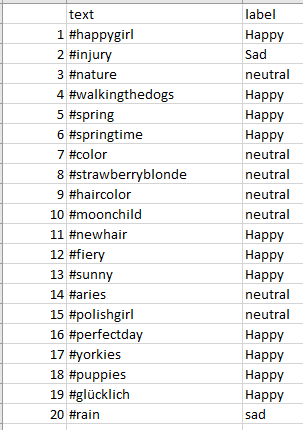
\includegraphics[width=6cm]{Dataset}
	\caption{Dataset Beispiel}
\end{figure}

Zunächst werden verschiedene imports gemacht, damit das Programm funktioniert. Um z.B. dann mit sklearn den TfidfVectorizer zu initialisieren.
\begin{lstlisting}
import numpy as np
import pandas as pd
import itertools
from sklearn.model_selection import 
train_test_split
from sklearn.feature_extraction.text 
import TfidfVectorizer
from sklearn.linear_model import 
PassiveAggressiveClassifier
from sklearn.metrics import accuracy_score,
confusion_matrix
\end{lstlisting}

Hier wird dann das Dataset eingelesen und in ein Dataframe gespeichert.
\begin{lstlisting}
#Read the data
df=pd.read_csv('C:\\Users\\Jonas Gerken
\\Desktop\\news.csv')

#Get shape and head
df.shape
df.head()
\end{lstlisting}


Dann werden die labels erstellt.
\begin{lstlisting}
#DataFlair - Get the labels
labels=df.label
labels.head()
\end{lstlisting}

Als nächstes wird das dataset in ein trainingsset und ein testingset aufgeteilt.
\begin{lstlisting}
#DataFlair - Split the dataset
x_train,x_test,y_train,y_test=train_test_split
(df['text'], 
labels, test_size=0.2, random_state=7)
\end{lstlisting}

An dieser Stelle wird dann der TfidfVectorizer mit stop words initialisiert.
Und der TfidfVectorizer wird in das trainings und testingset transformiert.
\begin{lstlisting}
#DataFlair - Initialize a TfidfVectorizer
tfidf_vectorizer=TfidfVectorizer(stop_words=
'english', max_df=0.7)

#DataFlair - Fit and transform train set, 
#transform test set
tfidf_train=tfidf_vectorizer.fit_transform(x_train) 
tfidf_test=tfidf_vectorizer.transform(x_test)
\end{lstlisting}

Im nächsten Schritt wird ein PassiveAggressiveClassifier initialisiert und wird auf tfidf train,y train angepasst.
Zuletzt wird die Genauigkeit des Test sets berechnet.

\begin{lstlisting}
#DataFlair - Initialize a PassiveAggressive
#Classifier
pac=PassiveAggressiveClassifier(max_iter=50)
pac.fit(tfidf_train,y_train)

#DataFlair - Predict on the test set and calculate 
#accuracy
y_pred=pac.predict(tfidf_test)
score=accuracy_score(y_test,y_pred)
print(f'Accuracy: {round(score*100,2)}%')
\end{lstlisting}\cite{b5}

\section{Zusammenfassung}
Zuletzt wird nochmal alles in einer Zusammenfassung kurz resümiert.
In der Ausarbeitung ging es um die Emotionserkennung basierend auf Sozialen Netzwerken.
Zunächst wurde erläutert was Emotionen sind.
Emotionen sind "ein mentaler und physiologischer Zustand, der mit einer Vielzahl von Gefühlen, Gedanken und Verhaltensweisen verbunden ist"
Des weiteren wurde beschrieben, das Emotionsanalysen zum Beispiel bei Erdbeben oder auch suizidalen Texten angewendet werden kann.
Es gibt verschiedene Emotionsmodelle, die zur Analyse verwendet werden. Hier zu gehört einmal Ekmans Modell mit seinen 6 Emotionstypen und das OCC-Modell, welches die Ekmans Emotionstypen beinhaltet, aber auch noch weitere dazugehören.
Weiter wurden Ansätze zur Emotionsanalyse erläutert, wie Keyword-basierter, lernbasierter und der hybridbasierte Ansatz. Der Keyword-basierte Ansatz basiert vollständig auf Schlüsselwörtern. Wiederum der lernbasierte Ansatz verwendet einen trainierten Klassifikator, um Eingabetext in Emotionsklassen zu kategorisieren, indem Schlüsselwörter als Merkmale verwendet werden.
Der dritte Ansatz kombiniert die ersten beiden Ansätze.
In der spezifischen Analyse von Emotionen in OSN Texten gibt es zwei Methoden. Einmal die lexikon basierte Methode, die auf Wörterbücher zurückgreift und die auf maschinellem Lernen basierenden Methoden, welche Emotionen normalerweise erkennen, indem sie Arten von Merkmalen aus Inhalten in OSNs extrahieren und dann Gefühle oder Emotionen unter Verwendung verschiedener Arten von Klassifizierungs- oder Regressionsmodellen vorhersagen.
Eine Anwendung ist die Analyse von Twitter Texten während eines Erdbebens. In dem Abschnitt wird beschrieben, was die Aufgaben, wie z.B. Tweets zu erkennen, die sich auf Erdbeben beziehen zu identifizieren, sind.
Emotionsanalyse kann auch im Bereich von suizidalen Texten verwendet werden. Hier wurden mehrere Abschiedsbriefe, halb echt, halb simuliert auf Merkmale analysiert um zwischen echten und gefälschten Notizen zu unterscheiden. Das schwierige ist das suizidale von normalen Sachen zu unterscheiden, da es zwischen bestimmten Sätzen Missverständnisse geben kann(z. B. ich würde mich nie umbringen versus ich werde mich umbringen oder das Verb hängen, um sich aufzuhängen versus Weihnachtslichter aufzuhängen). So kann es schnell zu falschen Entscheidungen kommen.
Im letzten Hauptabschnitt wurde dann ein Projekt zur Emotionserkennung durchgeführt. Dort wurde ein Dataset mit verschiedenen Emotionen erstellt. Über das Dataset konnte dann ein Maschine Learning System aufgebaut werden.


\begin{thebibliography}{00}
\bibitem{b1} X. Zhang, W. Li, H. Ying, F. Li, S. Tang and S. Lu, "Emotion Detection in Online Social Networks: A Multilabel Learning Approach," in IEEE Internet of Things Journal, vol. 7, no. 9, pp. 8133-8143, Sept. 2020
\bibitem{b2} H. Binali, C. Wu and V. Potdar, "Computational approaches for emotion detection in text," 4th IEEE International Conference on Digital Ecosystems and Technologies, 2010
\bibitem{b3} Collier, Nigel. “Twitter Emotion Analysis in Earthquake Situations.” 2013
\bibitem{b4} Desmet, Bart and Hoste, Véronique, Emotion detection in suicide notes", Expert Systems with Applications,
p. 6351–6358, 2013
\bibitem{b5} https://data-flair.training/blogs/advanced-python-project-detecting-fake-news/

\end{thebibliography}


\end{document}
